\subsection{Mächtigkeit von Mengen}
Für endliche (abzählbare) Mengen ist die Mächtigkeit gleichzusetzen mit der Anzahl
der Elemente einer Menge. Für unendliche (nicht abzählbare) Mengen müssen andere
Definitionen getroffen werden, um deren Mächtigkeit zu beschreiben.
\paragraph{Man schreibt:}
\({}|{}A{}|{}\) oder \(\#A\)
\paragraph{Es gilt:}
\begin{math}
{}|{}2^A{}|{} = 2^{{}|{}A{}|{}}
\end{math}

\paragraph{Satz von Cantor}
Die Mächtigkeit der Potenzmenge einer Menge A ist stets größer als die Mächtigkeit der Menge A selber:
$$ |2^A| > |A| $$
Dies gilt insbesondere für die leere Menge, da $2^0>0$.
Außerdem ist für sämtliche endliche Mengen klar: $ 2^n > n $.  Auch bei unendlichen Mengen lässt sich die Gültigkeit des Satzes zeigen.

\subsubsection*{Gleichmächtigkeit}
Seien A und B zwei beliebige Mengen.
Dann heißt A gleichmächtig zur Menge B, wenn eine Bijektion (\({f:A}\rightarrow{B}\)) gebildet
werden kann. Das bedeutet, dass eine Vorschrift existiert, welches
jedem Element der Menge A genau ein Element der Menge B zuordnet.
Dabei werden alle Elemente der Menge B einmal erfasst. Diese
Vorschrift ist umkehrbar.
\paragraph{Man schreibt:} \(\#A = \#B\) bzw. \(|A| = |B|\)
\paragraph*{Beispiele:}
\begin{math}
\#{\mathbb N} = \#{\mathbb Z} = \#{\mathbb Q}
\end{math}

Jede Menge, die gleichmächtig zur Menge der natürlichen Zahlen ist, wird als \emph{abzählbar} bezeichnet.
Die Mächtigkeit der reelen Zahlen hingegen wird als \emph{überabzählbar} bezeichnet.
\subparagraph{Erläuterung zu \(\#{\mathbb N} = \#{\mathbb Z}\):}
\begin{figure}[b]
  \centering
  \caption{Beispiel für eine Abbildung \(\#{\mathbb N} = \#{\mathbb Z}\)}
  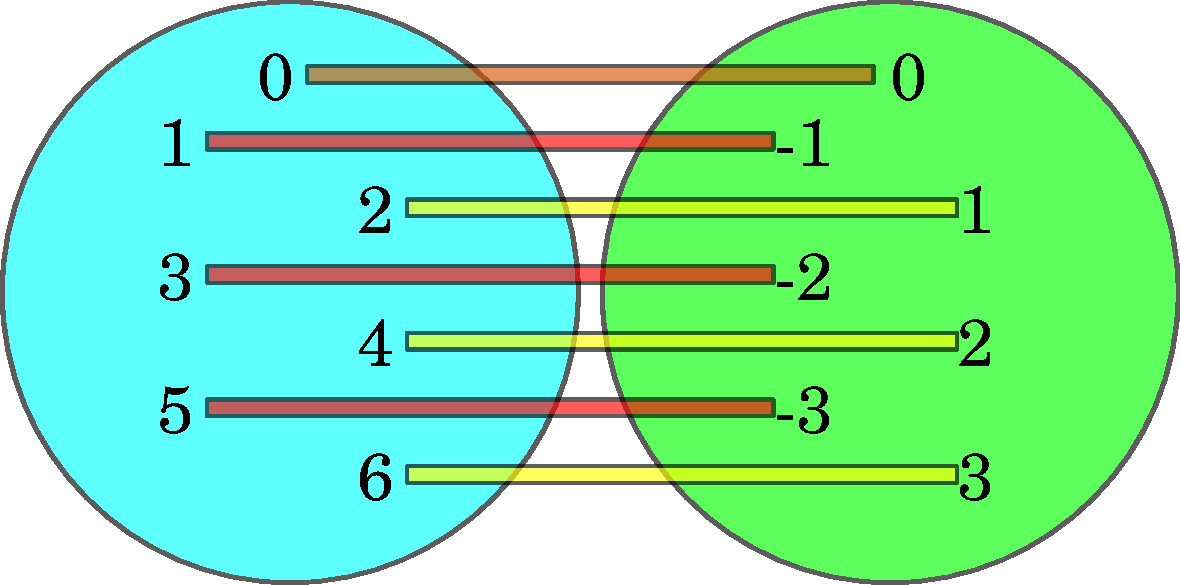
\includegraphics[scale=0.5]{ngleichz.pdf}
\end{figure}
Der Einwand, dass die natürlichen Zahlen doch ``offensichtlich'' (von der 0
abgesehen) doppelt so viele seien müssten, wie die ganzen Zahlen zählt
bei diesen unendlichen Mengen nicht! Stattdessen sollte man an die
Definition der Gleichmächtigkeit denken: 2 Mengen sind dann gleich,
wenn es eine eineindeutige(bijektive) Abbildung gibt.
Es werden also die 0 auf die 0, die ungeraden Zahlen auf die positiven
Zahlen und die geraden Zahlen auf die negativen Zahlen abgebildet.
Dies ist aufgrund der Unendlichkeit der beiden Mengen ohne Probleme
möglich.

Auch für die rationalen Zahlen lässt sich ein solches Schema für eine Bijektion finden.
Hierauf geht ein Wikipedia-Artikel näher ein:

% J.S.: Wir sollten die Wikipedia-Artikel später in das Skript einarbeiten..
\url{http://de.wikipedia.org/wiki/Cantors_erstes_Diagonalargument}

Und auch bei der Frage, warum die reellen Zahlen nicht abzählbar sind, hilft Wikipedia:

\url{http://de.wikipedia.org/wiki/Cantors_zweites_Diagonalargument}

% Quelle für nächsten Abschnitt: Repetorium höhere Mathematik, Merziger, Wirt, 6. Auflage, S.41 Aufgabe 1.60 und Lösung dazu
\subparagraph{Beispiel für überabzählbare Mengen}
Ähnlich wie beim vorherige Beispiel widerspricht es auch der Intuition, dass die Menge $\{ x | x \in (0,1) \}$ sowie $\{x | x \in {\mathbb R} \}$ gleichmächtig sind.
Schließlich ist das Intervall $(0,1)$ ja nur eine Teilmenge der reelen Zahlen.
\\Tatsächlich kann man schon mit Schulmathematik eine solche Bijektion finden: $$ f(x) = {1}/{\pi} * (arctan(x) + \pi/2 ) $$
Wer einen Blick auf den Graphen von $arctan(x)$ wirft wird dies schnell einsehen: 
die Funktion durchläuft sämtliche Werte von $-\infty$ bis $\infty$ und nimmt dabei nur Werte von $-\pi/2$ bis $\pi/2$ an. 
Durch Stauchung mit dem Faktor ${1}/{\pi}$ sowie Verschiebung nach oben kommt man dann zu obiger Funktion.

%%% Local Variables:
%%% mode: latex
%%% TeX-master: "../script"
%%% End:
